\chapter{Suggested method for importing FKB into OpenStreetMap}
Proof of concept 

\section{Method - Microtasking?}

% Går tilbake til metodene, hva kan vi lære i Norge hvor vi ikke har Mapbox. Norske FKB er bedre enn de man har importert i andre land
% Er dette beste metode?
%Hvordan dele opp i tasking områder? telle antall hus. 50-30-20 hus innenfor hver task? Dette er en utfordring, men er utenfor scopet til oppgaven. Komme med noen tanker rundt hvordan det kan løses. 


\section{FKB to OSM tagging}
%Hvilke tagger skal brukes for hva
%Skal vi bruke relations med 3D støtte? 

An example of a area representation of a building feature type is shown in listing \ref{eq:buildingfootpr}. This can be used as the building footprint when converting FKB to OSM. This will create the 2D modeling. Building type (BYGGTYP NBR) is equal to 111. The value 111 represents a house, so this building will be given a building=house tag. 

\lstset{
    language=XML,
    morekeywords={encoding,node, tag},
    label=eq:buildingfootpr,
    caption=Example of a area representation of a building feature type in SOSI. 
}
\begin{lstlisting}
.FLATE 715235:
..OBJTYPE Bygning
..KOMM 1601
..BYGGNR 182720836
..BYGGTYP_NBR 111
..BYGGSTAT TB
..KOPIDATA
...OMRÅDEID 1601
...ORIGINALDATAVERT "Trondheim kommune"
...KOPIDATO 20160502
..REF :166806
..NØ
703610900 55898600
\end{lstlisting}

\lstset{
    language=XML,
    morekeywords={encoding,node, tag},
    label=eq:buildingfootprline,
    caption=Example of a area representation of a building feature type in SOSI. 
}
\begin{lstlisting}
.KURVE 166806:
..OBJTYPE Takkant
..DATAFANGSTDATO 20100610
..VERIFISERINGSDATO 20150627
..REGISTRERINGSVERSJON "FKB" "4.01"
..KVALITET 24 19 0 24 23
..TRE_D_NIVÅ 2
..KOPIDATA
...OMRÅDEID 1601
...ORIGINALDATAVERT "Trondheim kommune"
...KOPIDATO 20160502
..NØH
703611202 55898706 1828 ...KP 1  
..NØH
703611328 55898445 1671
703610319 55897959 1671
703610193 55898220 1828 ...KP 1
..NØH
703610060 55898497 1671
703610540 55898728 1671 ...KP 1
..NØH
703610407 55899005 1671
703610668 55899130 1828 ...KP 1
..NØH
703610935 55899259 1671
703611065 55898990 1661 ...KP 1
..NØH
703611202 55898706 1828 ...KP 1
\end{lstlisting}

Using figure xx of the most common building types... Not all types used in FKB can directly translate to OSM. The tag-info page support searching for building values used in OSM. The most common FKB building types in OSM supported building values are shown in figure xx.


\section{Conversion using existing script}
% fkbbuilding.lua
%Lage utkast til en luafil, vise hvordan xml oppsettet blir 

The SOSI2OSM script was developed in 2013 and do not have any documentation. It is also difficult to install. It do not support SOSI files encoded in UTF-8, therefore the first step was to encode the FKB SOSI file into ISO8859-10 which is supported. %Er alle SOSI filer i UTF 8 idag?

It is not possible to get a 3D representation of the buildings with this script. Input is 


\section{How to map FKB buildings in 3D}
%Her kan jeg lage et eksempel på hvordan 3D bygg kan moduleres i OSM XML format. 
In order to create a XML representation capable of modeling FKB buildings in 3D, a standard approach should be developed. Members of the OpenStreetMap community, with interest in 3D mapping, started in March 2012 to unite all the separated approaches to model 3D buildings using OSM XML \cite{OpenStreetMapm}. They arranged workshops, which resulted in a suggestion for a simple 3D building schema. This is the approach mentioned in section \ref{buildOSM}. This approach is fairly easy to implement, if the building's roof shape is known. This is not the case for the FKB buildings, so the simple 3D building schema needs modification. Buildings in FKB is modelled with ridge and edge lines and they can be used to create 3D models, see the figures in section \ref{sec:FKBbuilding}. When using ridge and edge modeling roof shape tags are ignored, meaning the shape of the roof is not needed. Collecting ridge- and edge-lines for one building, creating one way-representation of each line with height-tags on ridge-lines. The listing shown in \ref{eq:3D_fkbbuilding} creates a 3D representation of a house in OSM from FKB data. The house is shown in figure \ref{fig:3DFKBbuild}, using the JOSM editor to generate the code in listing \ref{eq:3D_fkbbuilding} and getting 3D visualization.

\begin{figure}[H]
    \centering
    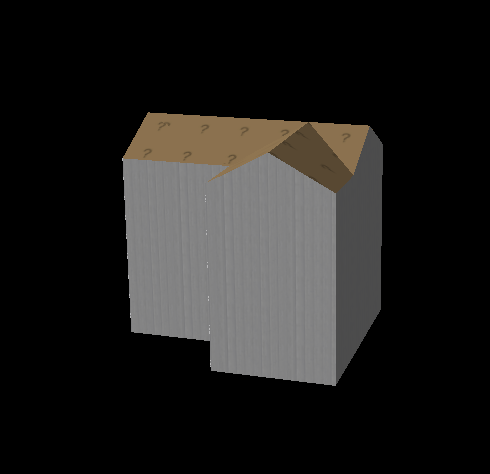
\includegraphics[scale=0.5]{figures/FixedByMe/3DFKBbuilding.png}
    \caption{3D representation of a FKB building, result of listing \ref{eq:3D_fkbbuilding}}
    \label{fig:3DFKBbuild}
\end{figure}

In OpenStreetMap, building height is the distance between the lowest possible position with ground contact and the top of the roof of the building, excluding antennas, etc \cite{OSMwikipage2016}. Height of buildings in FKB is height above sea level. This is a new challenge when mapping FKB buildings in OSM. In listing \ref{eq:3D_fkbbuilding} height above sea level is withdrawn from the height given from the FKB data. 

%The participants on the workshop agreed on building outlines should be used for the most general area of a complex building and building parts used to describe the special parts with different heights or other attributes, etc. As mentioned in section \ref{buildOSM}, the building outline should be tagged with building=* and building parts with building:part=*. Building outline is either a closed way or a multi-polygon and represents the area of land covered by the union of all building parts, the building footprint \cite{OSMwikipage2016}. Attributes like address, name, height, etc. must be tagged on the building outline. The building outline is important because it provides the compatibility for 2D rendering software. 2D renderers ignore building:part=* tags and only displaying the building outline. A relation tagged with type=building should be used if there are more than  one building part. This groups the building outline and all building parts together, as mentioned in section \ref{buildOSM}. 

There are different tools developed to visualizing 3D buildings with data from OSM. A problem is that not all tools supports the different modelling. A list of which of them who supports the simple 3D building schema is located at the OSM simple 3D buildings wiki page, most tools accept this schema. 7 tools supports building:part=yes %http://wiki.openstreetmap.org/wiki/3D_Development/Tagging#Usage_Community
2D renderers ignore building:part=* tags, only displaying the building outline. 

An example of 3D building generated from FKB data is shown in listing xx. This use the simple 3D building schema. 

\section{Evaluation}

